% Draft figure environments for author review; main.tex does not include them yet.
% Compile with the manuscript directory as the working directory.

\begin{figure}[t]
  \centering
  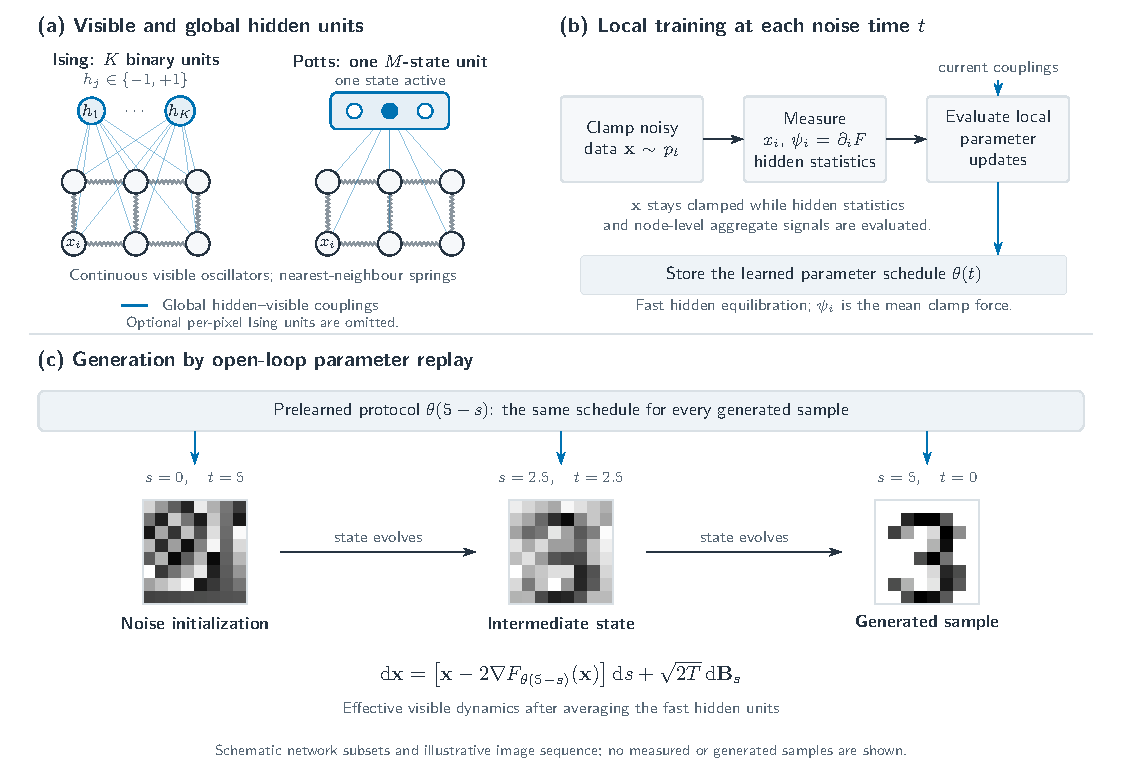
\includegraphics[width=\textwidth]{figures/conceptual_draft.pdf}
  \caption{\textbf{Local learning and open-loop generation with hidden degrees of freedom.}
  (a) Continuous visible oscillators with neighbour springs couple globally to
  either $K$ Ising units or one Potts unit with $M$ mutually exclusive states.
  Representative network subsets are shown; optional per-pixel Ising units
  are omitted. (b) At each noise time, visible units are clamped to noisy data.
  Mean clamp forces, conditional hidden statistics, node-level aggregate
  signals and current couplings determine local parameter updates.
  (c) Generation replays the learned schedule $\theta(5-s)$ while the visible
  state evolves from noise toward the data distribution. The displayed
  stochastic equation describes effective dynamics in the limit of fast hidden
  equilibration. The image sequence is an illustrative drawing, not simulation
  output.}
  \label{fig:latent_conceptual_draft}
\end{figure}

\begin{figure}[t]
  \centering
  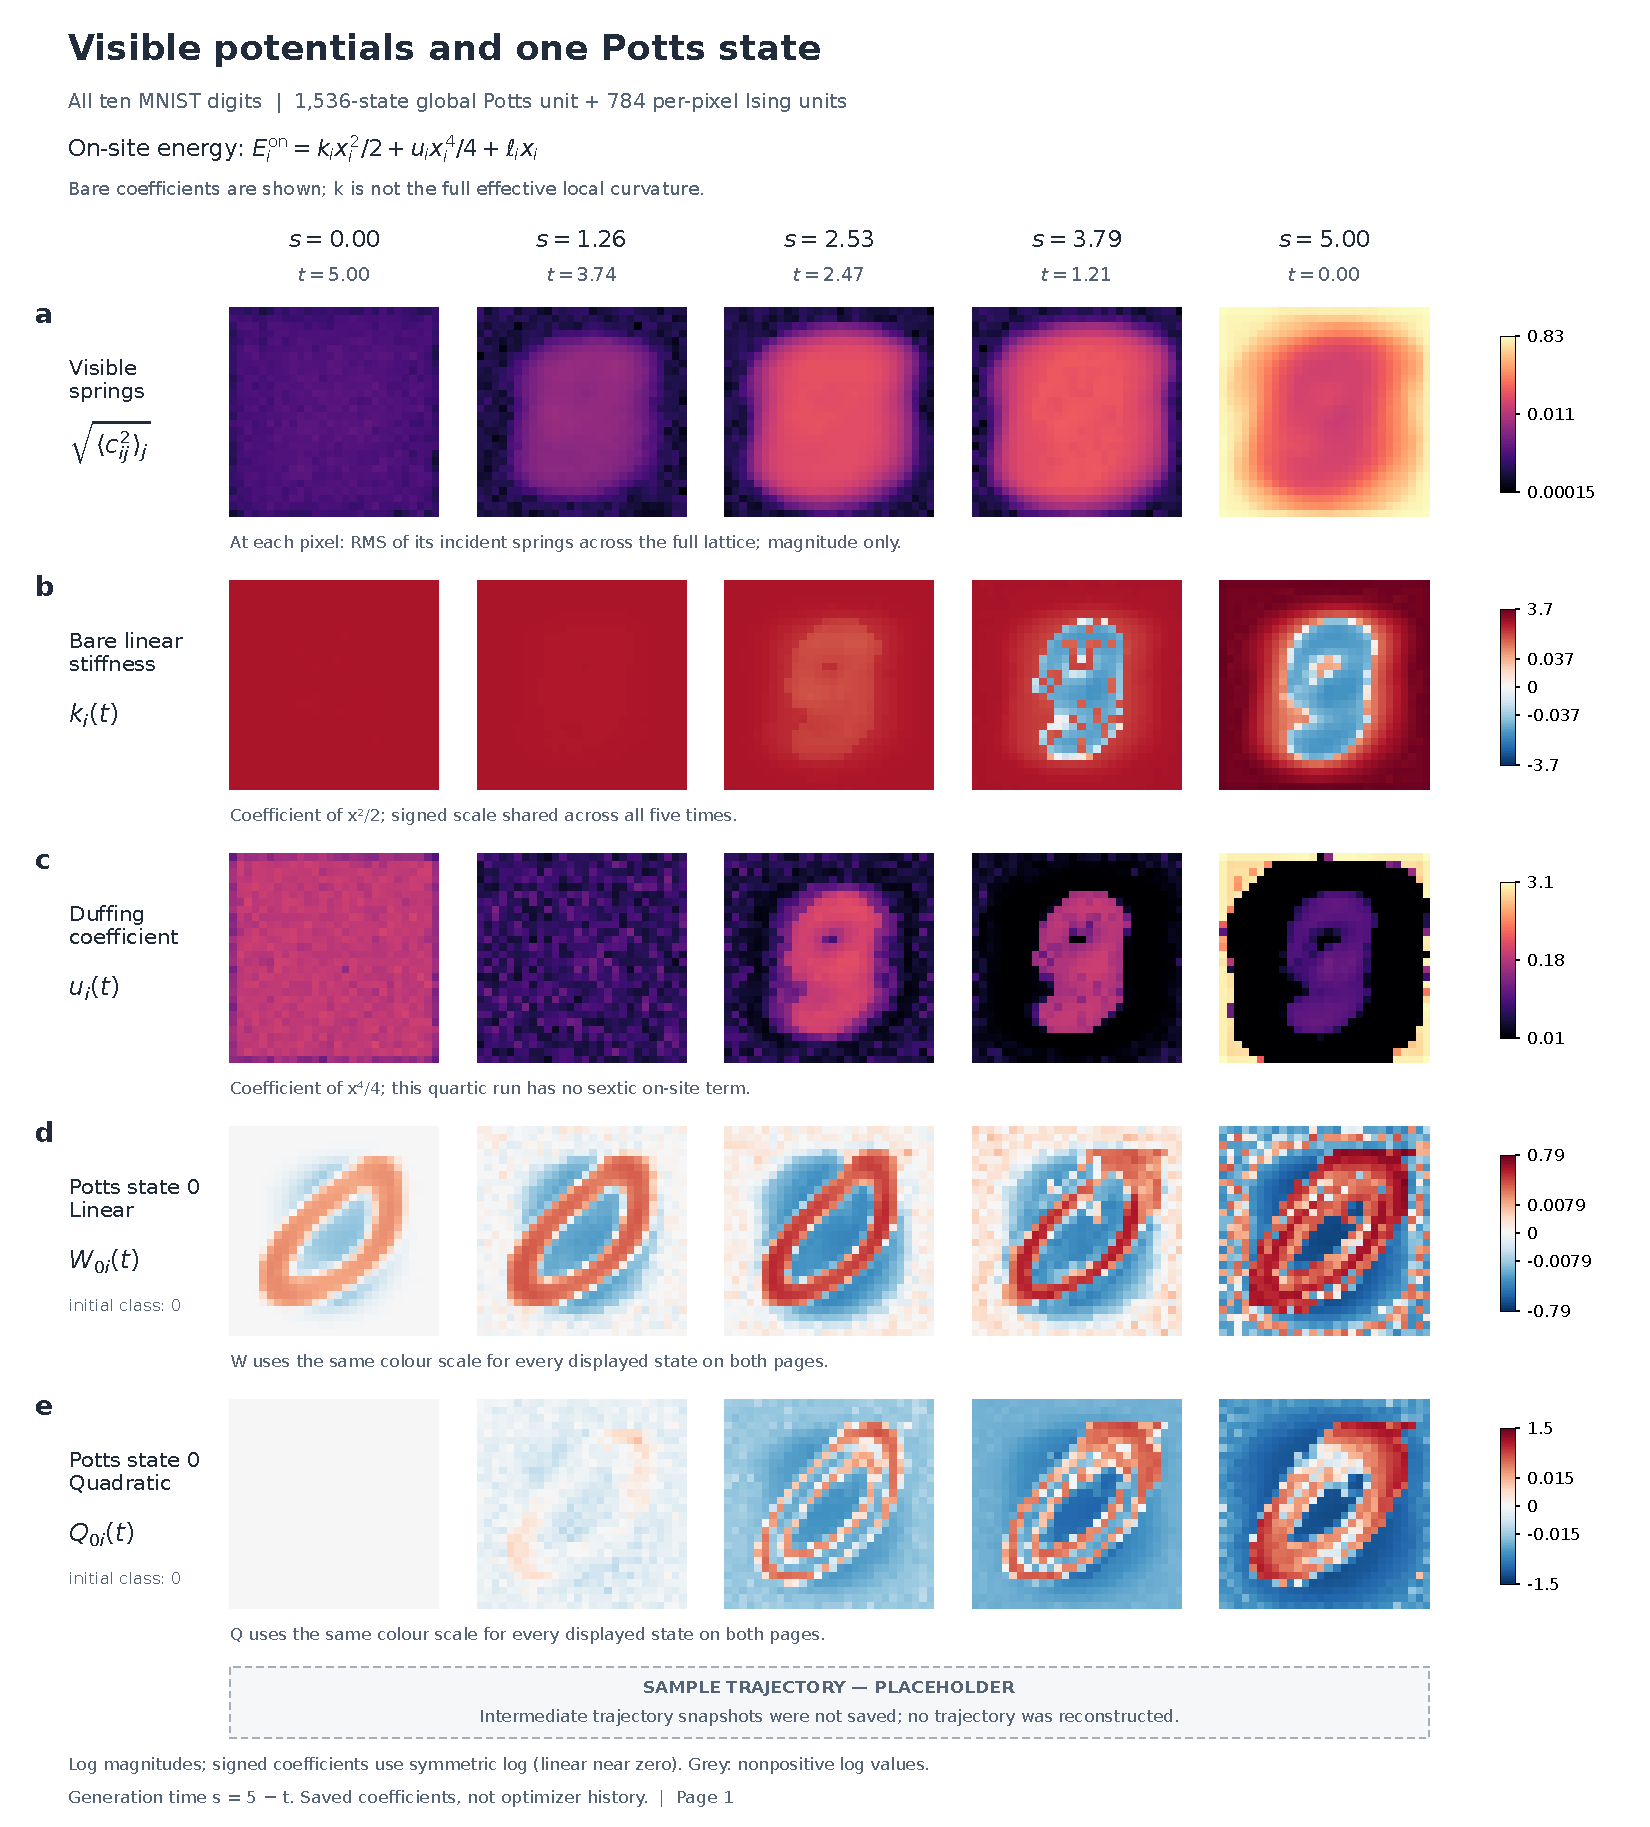
\includegraphics[page=1,width=\textwidth]{figures/parameter_evolution_draft.pdf}
  \caption{\textbf{A learned parameter schedule for generation.}
  Saved coefficients from the all-ten-digit MNIST model with one global Potts
  unit containing $1536$ states and $784$ per-pixel Ising units. Training used
  exact conditional hidden statistics. Columns follow generation time $s=5-t$,
  from the noisy end to the data end; this is not a record of optimizer steps.
  (a) Full-lattice maps of local spring magnitude. Each pixel $i$ shows
  $\sqrt{d_i^{-1}\sum_{j\in\mathcal{N}(i)}c_{ij}^2}$, where
  $d_i=|\mathcal{N}(i)|$ and $c_{ij}$ multiplies $(x_i-x_j)^2$.
  This quantity summarizes incident edges and does not retain their signs.
  (b,c) Bare on-site linear stiffness $k_i$ and Duffing coefficient $u_i$,
  defined by $E_i^{\mathrm{on}}=k_i x_i^2/2+u_i x_i^4/4+\ell_i x_i$.
  These coefficients are not the full effective curvature after including
  visible and hidden couplings. (d,e) Linear and quadratic
  coupling maps for the same Potts state (zero-based index $m=0$), entering
  $a_m(\mathbf{x})=b_m+\sum_i W_{mi}x_i+\sum_i Q_{mi}x_i^2$.
  The state index was fixed without selecting for sample quality or state
  occupancy. Positive spring magnitudes and Duffing coefficients use logarithmic
  colour scales. Signed coefficients use symmetric logarithmic scales with
  a linear interval around zero extending to $1\%$ of the maximum absolute
  displayed value for that parameter family. Each family has a common scale
  across all columns and, for $W,Q$, all four displayed states on both pages;
  raw coefficients are shown without removing the Potts common mode.
  Per-pixel hidden parameters, visible linear biases, hidden biases and
  the remaining Potts states are omitted. The trajectory panel is a placeholder:
  intermediate sample
  trajectories were not saved for this run.}
  \label{fig:parameter_evolution_draft}
\end{figure}

\begin{figure}[t]
  \centering
  \includegraphics[page=2,width=\textwidth]{figures/parameter_evolution_draft.pdf}
  \caption{\textbf{Three additional fixed Potts states.}
  Linear and quadratic coupling maps for state indices $j=1,2,4$, with the
  same time points and $W,Q$ colour scales as state $j=0$ on the preceding
  page. These three states were selected to include different initial cluster
  majority labels, respectively $6,2,9$. Initialization labels are diagnostic
  annotations, not measurements of final learned-state class purity.
  The patterns show raw saved coefficients, without common-mode removal or
  normalization of individual states or frames.}
  \label{fig:additional_potts_states_draft}
\end{figure}

\begin{figure}[t]
  \centering
  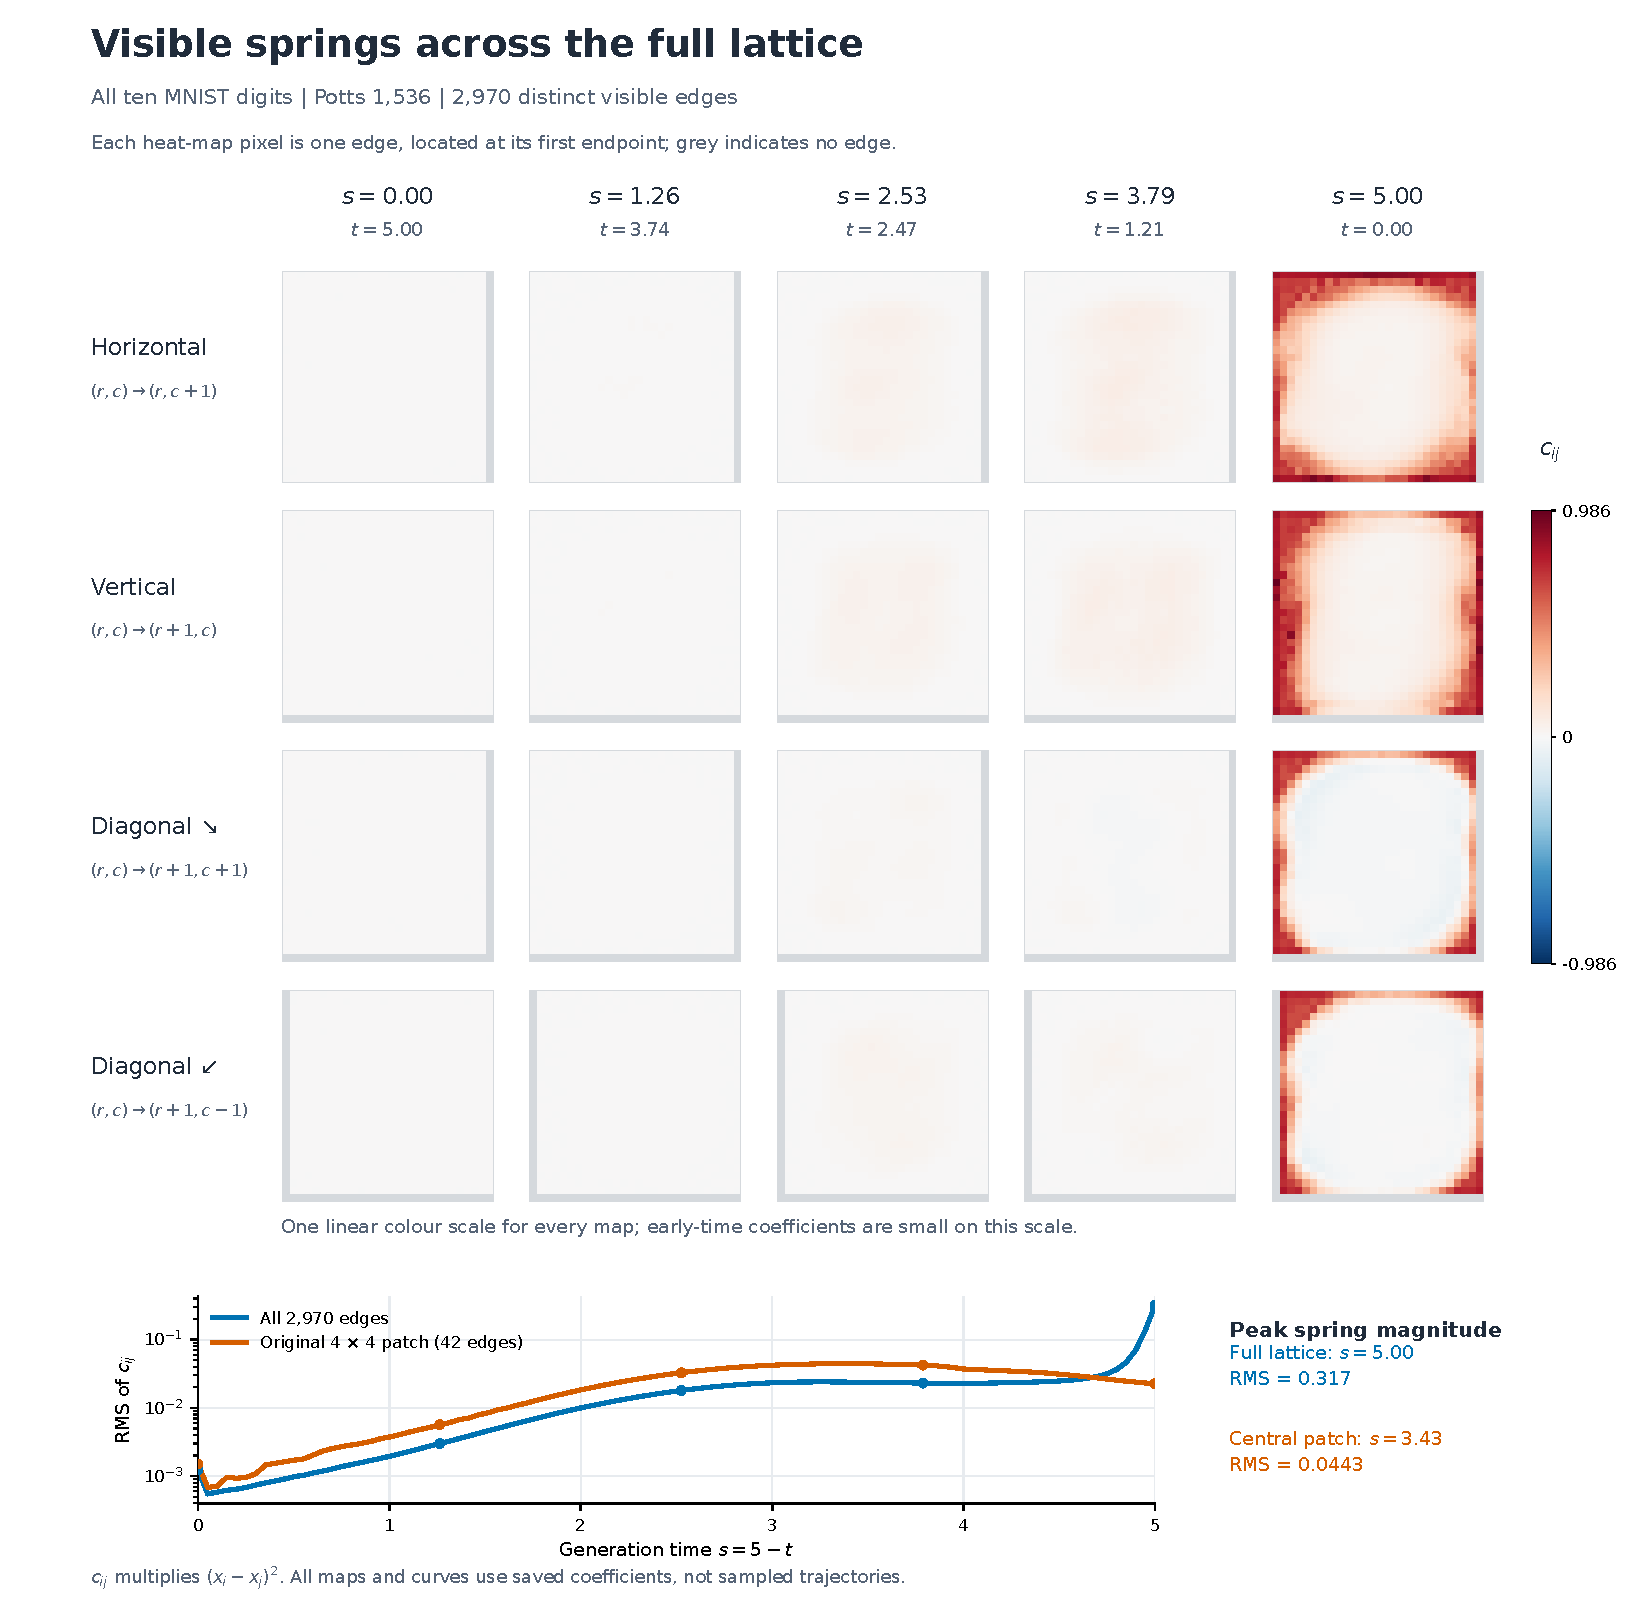
\includegraphics[width=\textwidth]{figures/visible_coupling_evolution.pdf}
  \caption{\textbf{Spatial structure of the visible spring schedule.}
  Signed spring coefficients are separated into horizontal, vertical and two
  diagonal orientations so that each edge appears once. The maps use a common
  colour scale across orientations and displayed times. Strength curves show
  root-mean-square coefficients over all $2970$ edges and over the $42$ edges
  in the central $4\times4$ patch used in the initial graph draft. The
  central patch weakens near the data end, whereas the full-lattice RMS is
  largest at the final time. These are learned coefficient schedules, not
  measurements of trajectory-dependent forces or a controlled explanation
  of the sampling dynamics.}
  \label{fig:visible_coupling_evolution_draft}
\end{figure}
